\documentclass[sigconf,10pt,nonacm]{acmart}

\hfuzz=100pt
\hbadness=99999
\vbadness=99999

\renewcommand\footnotetextcopyrightpermission[1]{}

\pdfstringdefDisableCommands{%
  \def\\{}%
}

\usepackage{hyperref}
\usepackage{listings} %%to import the svg circuit scheme 
\usepackage{float}


%% \BibTeX command to typeset BibTeX logo in the docs
\AtBeginDocument{%
  \providecommand\BibTeX{{%
    Bib\TeX}}}

%% Rights management information.  This information is sent to you
%% when you complete the rights form.  These commands have SAMPLE
%% values in them; it is your responsibility as an author to replace
%% the commands and values with those provided to you when you
%% complete the rights form.
\setcopyright{acmlicensed}
\copyrightyear{2024}
\acmYear{2024}
\acmDOI{XXXXXXX.XXXXXXX}


\begin{document}

\title{Slideshow remote provided with TinyML \& USB HID control on Arduino Nano 33 BLE sense}

\author{Titien MARIE \\ Erasmus Student}
\email{titienjacques.marie@unitn.it }
\orcid{123}


\affiliation{%
  %\institution{Department of Information Engineering and Computer Science}
  \institution{University of Trento}
  \streetaddress{Via Sommarive 9}
  \city{Povo}
  \state{Trento}
  \country{Italy}
  \postcode{38123}
}

\renewcommand{\shortauthors}{Titien Marie}


\begin{abstract}
Gesture-based human-computer interaction offers intuitive and hands-free control for various applications. However, existing solutions often rely on expensive hardware or complex setups, limiting their accessibility. This work presents a low-cost/power gesture-controlled presentation remote built on an Arduino Nano 33 BLE, combining TinyML-based gesture recognition with USB HID control.
Our key insight is that embedding a TensorFlow Lite Micro classifier directly on a microcontroller enables real-time gesture recognition without external computation, while USB HID allows seamless integration with any host system. The system extracts 42 statistical and spectral features from IMU data (accelerometer and gyroscope) across 128 samples, classifies gestures among four classes (left, right, rest, shake), and maps them to keyboard events (arrow keys, Home).
The main artifacts include the embedded C++ classifier running on-device, a Python data collection pipeline, and a physical prototype with an external button with physical button input handling. Results demonstrate reliable gesture classification and responsive HID control, enabling hands-free PDF navigation on macOS via the Preview application or Keynote/PowerPoint.
\end{abstract}

\maketitle
%
%I \emph{recommend}---but do not require--- that you use
%the following organization for your abstract. 
%Sections~\ref{sec:motivation} through \ref{sec:key-contributions}
%should be a summary of your full paper. Section~\ref{sec:motivation}
%motivates the paper; Section~\ref{sec:limitations} describes
%limitations of the state of the art, if applicable;
%Section~\ref{sec:key-insights} presents the key new insight or
%insights of the paper; 
%Section~\ref{sec:main-artifacts} presents the main artifacts described
%in the paper;  Section~\ref{sec:key-contributions} summarizes the key
%results and technical contributions of your paper. 
%
%\begin{itemize}
%    \item Your paper should be {\bf minimum 4} pages.
%
%    \item You will submit your paper via {\bf \href{https://unitn-lpes24.hotcrp.com/}{https://unitn-lpes24.hotcrp.com/}}
%\end{itemize}


\section{Motivation}
\label{sec:motivation}

Traditional presentation remotes are either expensive, proprietary, or limited to simple next/previous slide controls. They rely on dedicated Radio Frequency or Bluetooth hardware, require drivers, and offer no extensibility for custom gesture-based interactions. Meanwhile, embedded machine learning has made it possible to run neural network inference directly on microcontrollers, opening new possibilities for low-cost, low power (\textit{if optimized}) intelligent input devices.
This work addresses the problem of building an affordable, gesture-controlled presentation remote using commodity hardware and open-source tools (\textit{C++, Python, PlateformIO, Arduino documentation}). The device must recognize natural hand gestures in real time efficiently, map them to keyboard events, and integrate with any operating system without additional software, a combination that existing solutions do not offer at low cost.
This is an important problem because presentation tools are everywhere and necessary in academic and professional settings, yet intuitive hands-free control remains inaccessible to most users due to cost or technical complexity such as : provided uniquely for a specific Operating System, installation of specific drivers, updates... A sub-50€ solution built on a widely available microcontroller, basic components, and open-source tools provides an accessible alternative to existing proprietary remotes on the market. 


%
%\section{Limitations of the State of the Art}
%\label{sec:limitations}

%\begin{itemize}
%\item What is the state of the art in this topic today (if any)?
%\item What are its limits?
%\end{itemize}

\section{Key Insights}
\label{sec:key-insights}

The first key insight is that TinyML  can be embedded directly on a low-cost microcontroller (Arduino Nano 33 BLE \cite{arduino_nano}) to perform real-time gesture classification without any external computation. By extracting 42 statistical and spectral features from raw IMU data and running a TensorFlow Lite Micro (\cite{tensorflow_lite})model on-device, the system achieves responsive gesture recognition within a tight memory and power budget.
The second key insight is that USB HID provides a universal, driver-free interface between the device and any host operating system. By sending raw HID reports directly, bypassing the keymap layer provided natively by Mbed for ARM (\cite{mbed}) architecture, the system overcomes keyboard layout dependencies (e.g. AZERTY and QWERTY) and reliably sends special keys such as arrow keys and Home, which standard Arduino keyboard libraries fail to handle correctly.
Together these two insights enable a self-contained, plug-and-play gesture remote that requires no dedicated software, no Bluetooth pairing, and no proprietary receiver theoretically. On the other hand, as this solution is recognized by the Operating System (\textit{as we have experienced on MacOS} )as an external USB device it requires the accessibility authorization of the user where without it we can not guarantee the whole functionality and availability of our remote.   




\section{Implementation}
\label{sec:implementation}
Firstly, in order to get the Arduino usable for further projects and same for the components we used a basic breadboard with some \textit{Dupont wires} where we plugged the microcontroller directly on it , for GND, VCC (\textit{3.3V}) and the D11 reception, we added an external push button connected to the pin 11 of the Arduino with a 10 $k \Omega$  pulldown resistor to avoid  interference and unwanted behavior.  Then to improve the user experience we added a LED. 
Then, the usage of PlatformIO \cite{platformio} helps us to provide a program that can be portable with specific building flags and library dependencies : we choose the Arduino 33 BLE Sense without Revision and the Rev2. Inside each \textit{version} of the Arduino we provided two environment  that can be transmitted to it : \texttt{Collect\_Data} that can give to the user the accelerometer coordinates (\texttt{aX,aY,aZ}) and the gyroscope (\texttt{gX,gY,gZ})  and the default one that has no name in our implementation (\textit{the name of the Arduino presently}). \newline 
You will see below some pictures about the circuit diagram and the real physical implementation. 

\begin{figure}[!t]
    \centering
    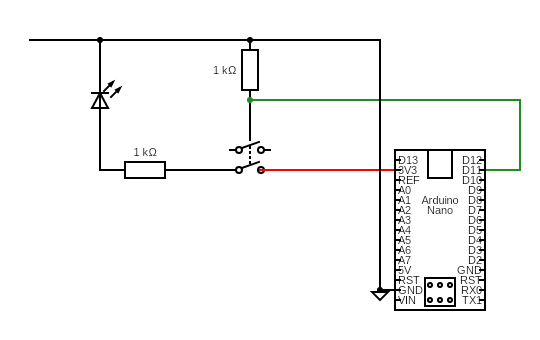
\includegraphics[width=\linewidth]{circuit.png}
    \caption{Circuit diagram (via \cite{circuit_diagram}) of the gesture remote prototype}
    \label{fig:schema}
\end{figure} 

In this scheme, the Arduino Nano 33 BLE is directly linked to the user computer via an USB type A to microUSB cable that provides the 5V power distributed to 3.3V into the breadboard , In other words inside the Arduino an onboard voltage regulator steps down the supply to 3.3V, which is distributed to the external components through the VCC pin. It is important to note that all GPIO pins on the Nano 33 BLE are 3.3V tolerant only, applying 5V directly to any GPIO pin may permanently damage the microcontroller.  The resistors can be changed depending on the necessity of the user\textit{ (LED luminance, reactivity...) }
Here the Ground is common, same for the VCC due to the breadboard implementation. To get into more details we provide few pictures.

\begin{figure}[!t]
    \centering
    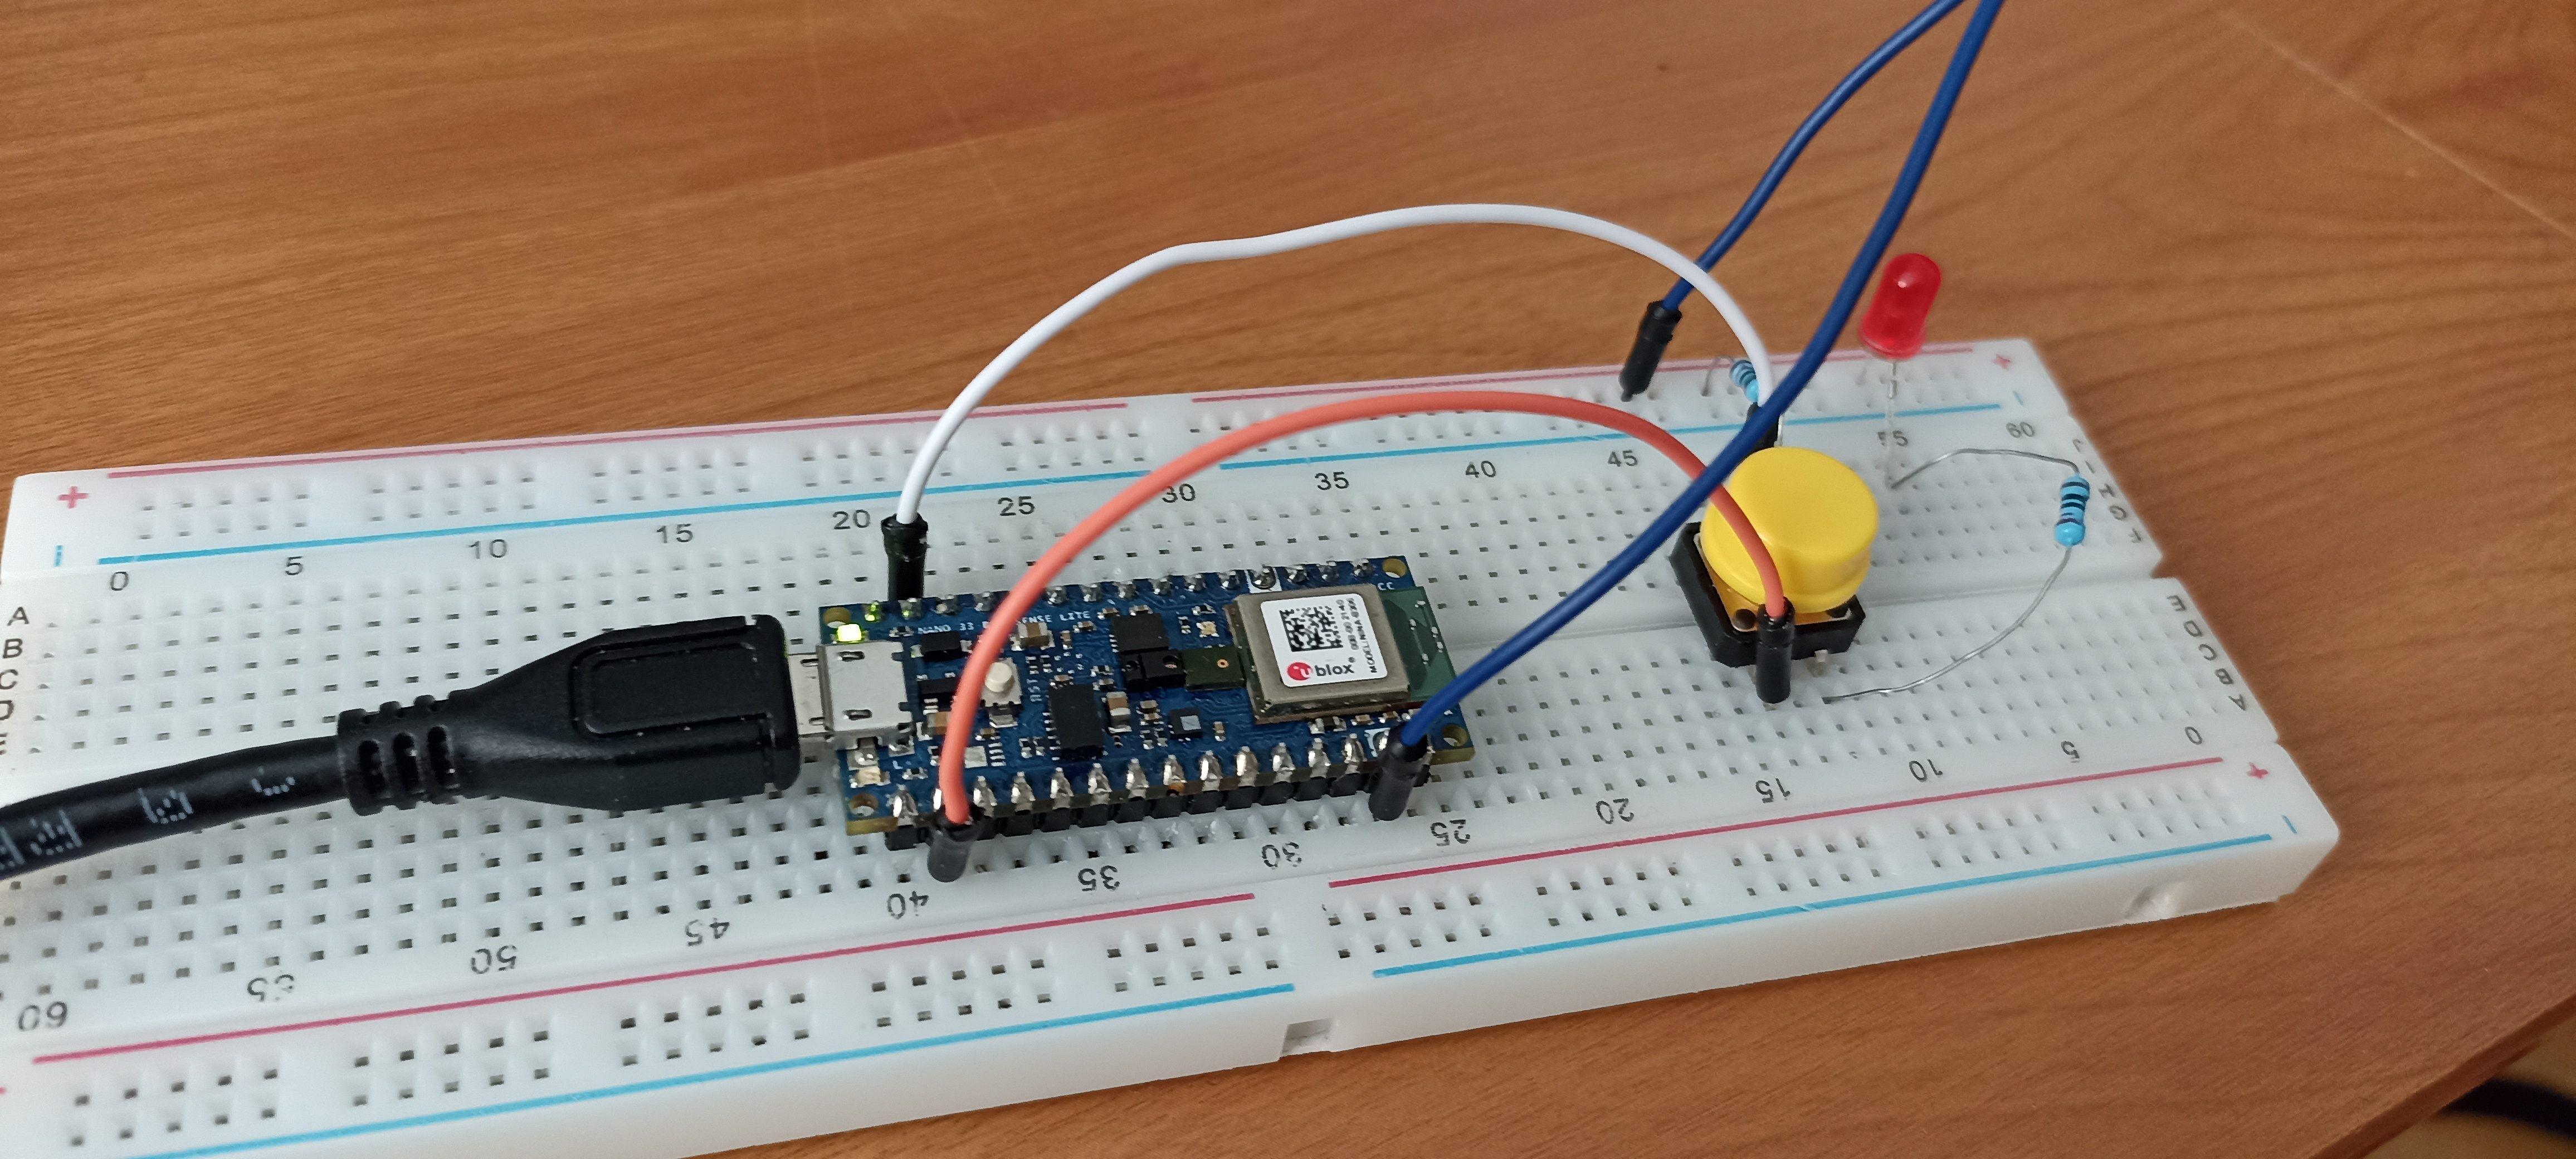
\includegraphics[width=\linewidth]{implementation-1.jpg}
    \caption{The overall of the remote}
    \label{fig:schema2}
\end{figure} 



\begin{figure}[!t]
    \centering
    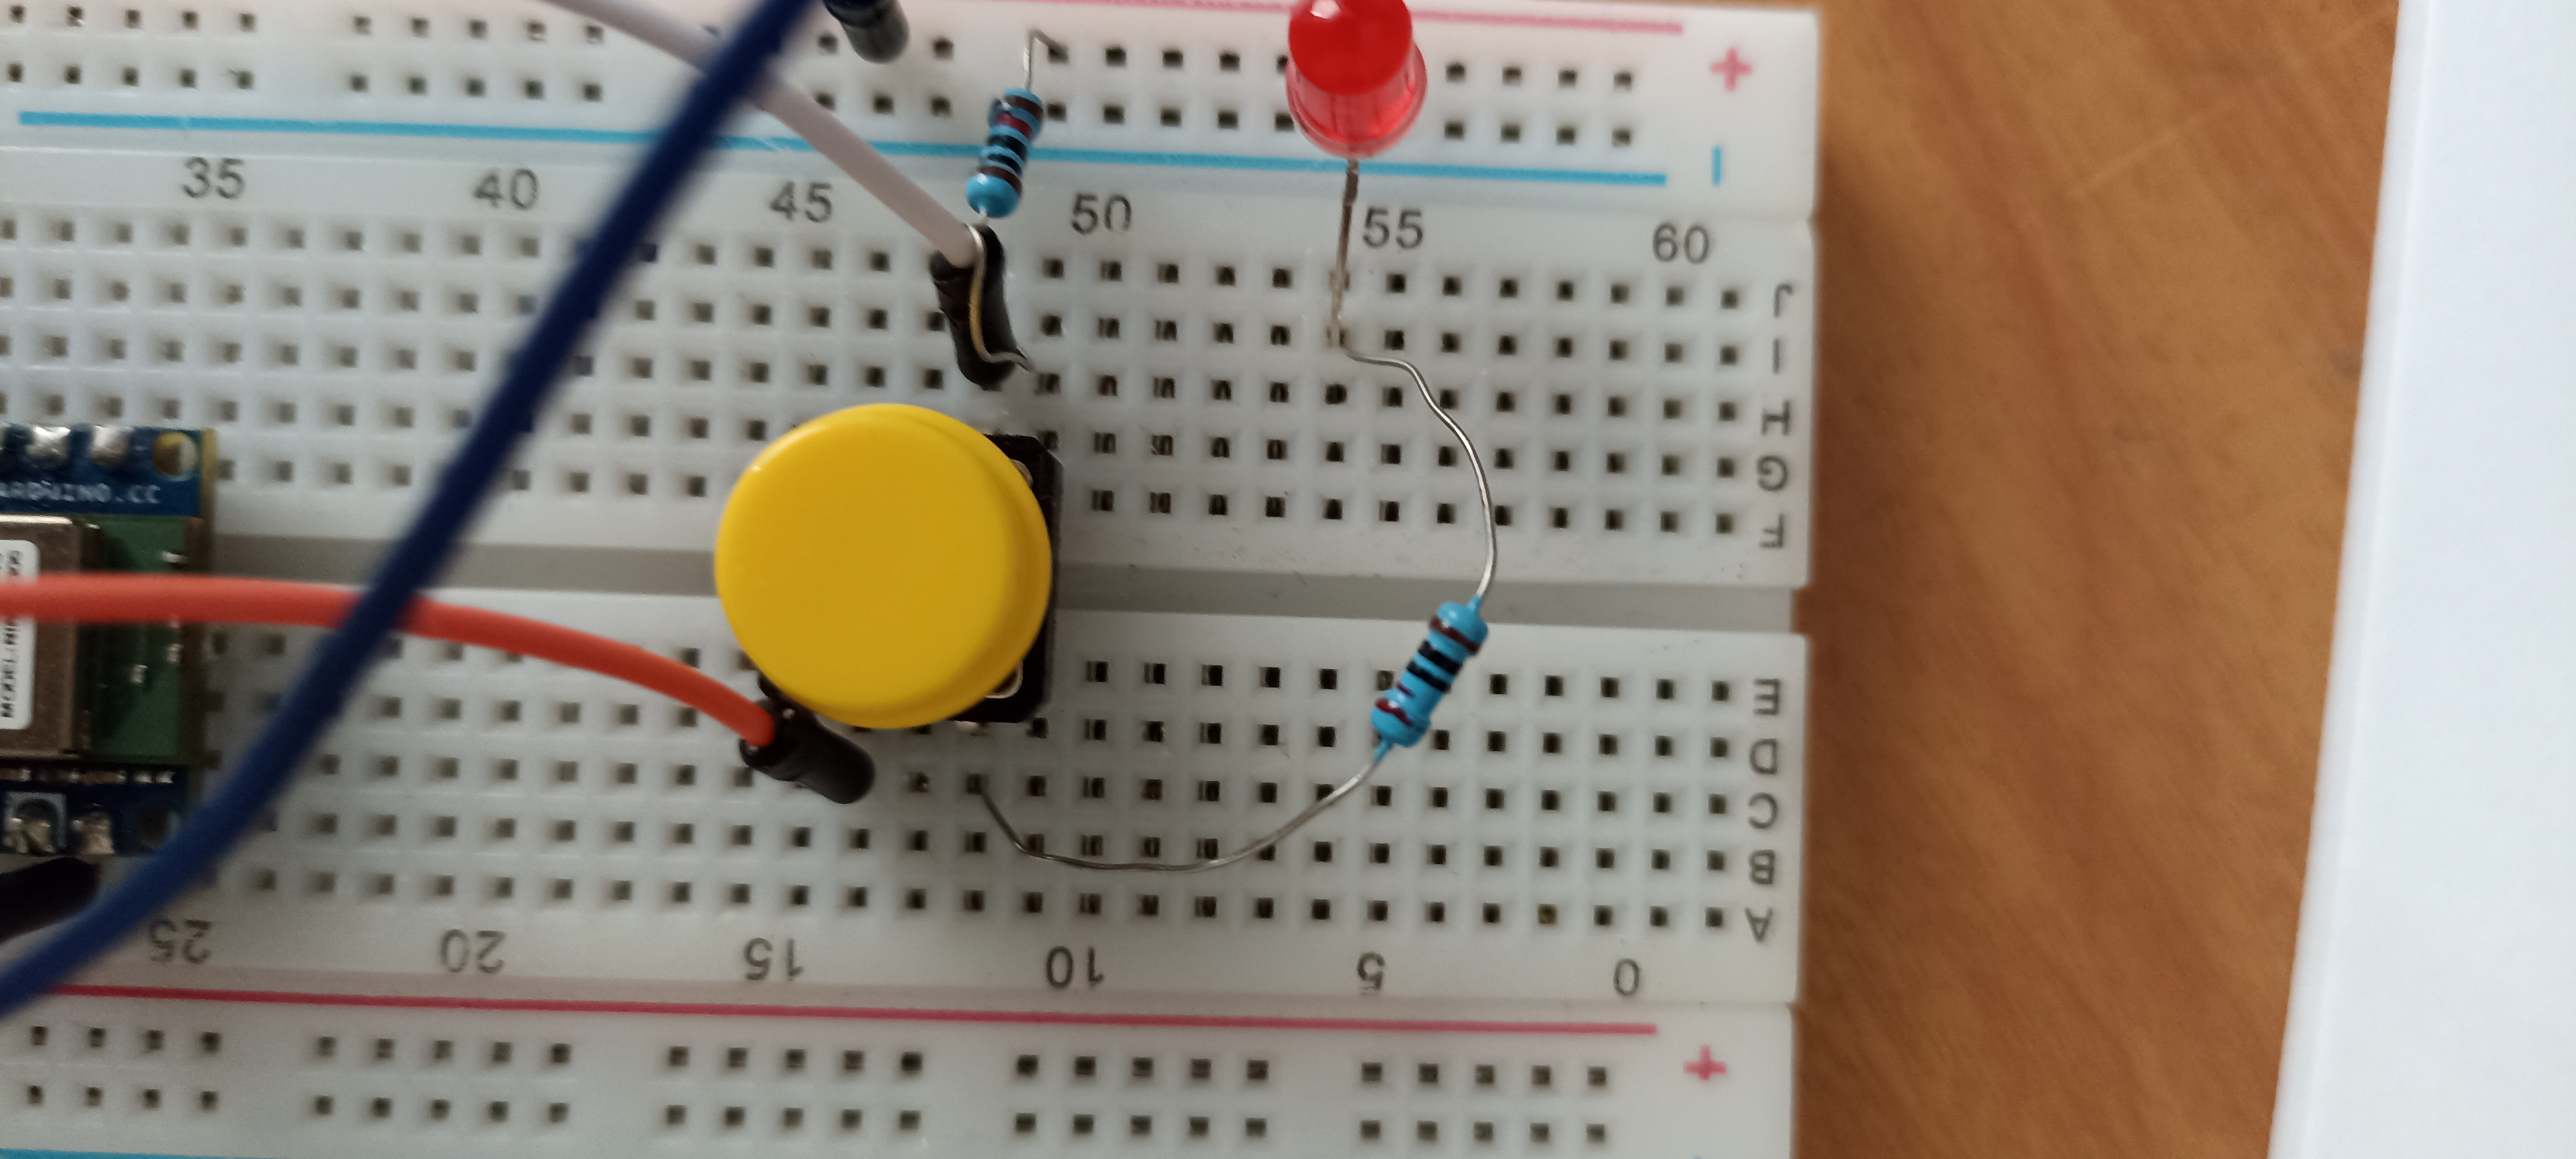
\includegraphics[width=\linewidth]{implementation-3.jpg}
    \caption{More details on the components}
    \label{fig:schema3}
\end{figure} 

As we would like to re-use the Arduino we did not solder it or covered the different layers.
Now, we can go deeper in the inter implementation.  
\subsection{Feature Extraction}
For each of the 6 IMU axes  7 statistical and spectral features are extracted from a window of 128 samples : mean, standard deviation, RMS (\textit{Root Mean Squared}) , minimum, maximum, PSD (\textit{Power Spectral Density}) mean and PSD max (computed via FFT directly on the Arduino via the proper library), resulting in 42 features total. These features are then normalized and fed into the TensorFlow Lite Micro model for inference.

\subsection{TinyML Pipeline}
The gesture recognition pipeline follows three steps. First, data is collected using the \texttt{COLLECT\_DATA} build flag (\textit{see \ref{sec:implementation}}), which enables the Arduino to stream the 42 extracted features per gesture over Serial to the host computer. A Python script captures this data and saves it as a labeled CSV file, one per gesture class. Second, a neural network classifier is trained offline on the collected dataset using TensorFlow/Keras on the host computer. Finally, the trained model is converted to a TensorFlow Lite Micro format and embedded as a \texttt{model.h} C++ header file, which is compiled directly into the firmware and defines the different parts of the program that corresponds either to \texttt{COLLECT\_DATA} or the inference one .

\subsection{USB HID Bypass}
As mentioned in Section~\ref{sec:key-insights}, the standard Arduino keyboard library relies on a keymap table to translate ASCII character indices into HID usage codes (\textit{see HUT keyboard usage table, section 10 \cite{Hut})} . However, special keys such as arrow keys and Home have indices that exceed the keymap size (152 entries), making them unreachable via the standard API. To overcome this, we implement a \texttt{sendKey()} function that constructs and sends raw HID reports directly, bypassing the keymap entirely :

\begin{lstlisting}[language=C++, caption=Raw HID report bypassing the keymap]
report.data[0] = 0x01; // REPORT_ID_KEYBOARD
report.data[3] = hidCode; // direct HID  code
key_mouse.send_nb(&report);
\end{lstlisting}

This approach is layout-independent and works regardless of whether the host uses AZERTY, QWERTY, or any other keyboard layout.

\subsection{Gesture to Key Mapping}
Table~\ref{tab:mapping} summarizes the mapping between recognized gestures and the corresponding keyboard events sent to the host.

\begin{table}[H]
\centering
\caption{Gesture to keyboard mapping}
\label{tab:mapping}
\begin{tabular}{c | c | c |}
\hline
\textbf{Gesture / Input} & \textbf{Key sent} & \textbf{Keycode} \\
\hline
Left gesture  & $\leftarrow$ (previous slide) & 0x50 \\

Right gesture & $\rightarrow$ (next slide) & 0x4F\\
Shake gesture & Home (first slide) & 0x4A \\
Physical button  & $\rightarrow$ (next slide) & 0x4F \\
\hline
\end{tabular}
\end{table}



%\begin{itemize}
%\item What are the one or two key new insights in this paper?
%\item How does it advance the state of the art?
%\item What makes it more effective than past approaches?
%\end{itemize}

\section{Main Artifacts}
\label{sec:main-artifacts}

This work produces three main artifacts:

\begin{itemize}
    \item \textbf{Embedded firmware (C++)} : a self-contained Arduino firmware 
    that reads IMU data, extracts 42 statistical and spectral features, runs a 
    TensorFlow Lite Micro classifier on-device, and sends raw USB HID reports 
    to the host. The firmware supports two build environments via PlatformIO : 
    a data collection mode (\texttt{COLLECT\_DATA}) and an inference mode.

    \item \textbf{Data collection and training pipeline (Python)} : a Python 
    script that captures labeled gesture data over Serial and saves it as CSV 
    files. A separate training script uses TensorFlow/Keras to train a neural 
    network classifier and exports it as a \texttt{model.h} header file ready 
    to be compiled into the firmware.

    \item \textbf{Physical prototype} : a breadboard-based prototype featuring 
    an Arduino Nano 33 BLE, an external push button with a 10~$k\Omega$ 
    pulldown resistor, and a red LED for visual feedback. The device connects 
    to any host computer via USB and requires no additional drivers or software theoretically.
\end{itemize}

The artifacts were evaluated by testing the gesture recognition accuracy on four gesture classes (left, right, rest, shake) and verifying the correct 
transmission of HID keyboard events on macOS using the Preview and Keynote 
applications.

\section{Key Results and Contributions}
\label{sec:key-contributions}

\subsection*{Key Results}
The system successfully classifies four gesture classes in real time directly 
on the Arduino Nano 33 BLE, with no external computation required. The USB HID 
interface reliably sends special keyboard events (arrow keys and Home) to 
the host regardless of the keyboard layout configured on the operating system, 
which standard Arduino libraries fail to achieve.

\subsection*{Contributions}

\begin{itemize}
    \item \textbf{On-device TinyML gesture recognition} : we demonstrate that 
    a TensorFlow Lite Micro classifier trained on 42 IMU-derived features can 
    run reliably on a Cortex-M4 microcontroller with 256~KB of RAM, enabling 
    real-time gesture classification. 

    \item \textbf{Layout-independent USB HID control} : we identify and solve 
    a fundamental limitation of the standard Arduino keyboard library, whose 
    keymap table truncates special key indices. By constructing raw HID reports 
    directly based on the USB HID Usage Tables specification 
    \cite{HUT}, we achieve layout-independent key transmission 
    compatible with any operating system.

    \item \textbf{Low-cost, open-source presentation remote} : the complete 
    system, hardware, firmware, and training pipeline,  is built exclusively 
    from commodity components and open-source tools, for under 50€, providing 
    an accessible alternative to proprietary gesture remotes on the market.
\end{itemize}

\subsection*{Advantages over existing approaches}
Existing presentation remotes rely on proprietary RF or Bluetooth receivers, 
require OS-specific drivers, and offer no gesture extensibility. Our solution 
requires only a standard USB connection,  and allows users to retrain the gesture classifier for custom interactions using the provided Python pipeline.

\section{Possible improvements} 
This other advantage of this projets is also that it is not fixed, it can be improved for further works, where here you can find some examples : 

\begin{itemize} 
	\item We tried to implement an ISR (\textit{Interrupt Service Routine}) to give to the external push button the priority on the execution . In this way it can stop the inference or the data collection in order for the user to not feel the weight of the TinyML. We did not succeed to implement due, maybe to the board that is not efficient with this type of interruption. In our case, we had only one interruption at the first time we push the button and then it is completely ignored. \\
	\item If we want to something wireless, it may be possible to implement our solution without USB HID but via Bluetooth (BLE) HID with a battery directly linked to the board using appropriate connectors. \\
	\item To get a better User Experience (UX) we can add more gestures and other external components into our remote : such as a laser pointer or by using the voice recognition. \\
	\item In the same way as previously, we can add an haptic feedback (vibration) and maybe different souds with a passive/active buzzer for a better accessibility. \\
	\item Finally, we can try our model on other Operating Systems to guarantee the compatibility and portability for all types of users (\textit{programmers, students, workers...) } 
	
\end{itemize}


\section*{Acknowledgements}
We would like to thank Alan MASUTTI for his  
contribution to this project, particularly for the writing of the PlatformeIO environment and the main file organization. 
Finally we also thanks M. Sinan , for his  guidance and supervision throughout this work.

\bibliographystyle{plain}
\bibliography{references}
\end{document}



